% Intended LaTeX compiler: pdflatex
\documentclass[letterpaper]{article}
\usepackage[utf8]{inputenc}
\usepackage[T1]{fontenc}
\usepackage{graphicx}
\usepackage{grffile}
\usepackage{longtable}
\usepackage{wrapfig}
\usepackage{rotating}
\usepackage[normalem]{ulem}
\usepackage{amsmath}
\usepackage{textcomp}
\usepackage{amssymb}
\usepackage{capt-of}
\usepackage{hyperref}
\usepackage{pgfplots}
\usepackage{pdfpages}
\usepgfplotslibrary{groupplots}
\usepackage[american,siunitx]{circuitikz}
\usetikzlibrary{arrows,shapes,calc,positioning}

\author{Kjartan Halvorsen}
\date{\today}
\title{PI \& D exercise}

\begin{document}

\maketitle

\section*{Example 1}
\begin{center}
  \begin{tikzpicture}
    \tikzset{
      every pin/.style={pin distance=2cm,fill=blue!20!white,rectangle,rounded corners=3pt,font=\small,
      align=left},
    small dot/.style={fill=black,circle,scale=0.3},
  }

    \node {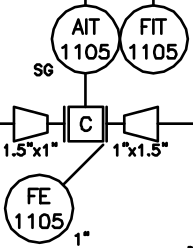
\includegraphics[width=0.25\linewidth]{../../figures/PInD-ex1.png}};

    %\foreach \x in {-2, -1.5,...,2} \draw[thin, black!30] (\x,-2) to (\x, 2);
    %\foreach \y in {-2, -1.5,...,2} \draw[thin, black!30] (-2,\y) to (2,\y);

    \node[coordinate,pin=170:{Specific gravity}] at (-1,1) {};
    \node[coordinate,pin=190:{Pipe diameter reduced\\ from 1.5in to 1in}] at (-1,0) {};
    \node[coordinate,pin=-30:{Pipe diameter increased\\ from 1in to 1.5in}] at (0.7,0) {};
    \node[coordinate,pin={[pin distance=3cm]-80:{Coriolis effect element}}] at (0,0) {};
    \node[coordinate,pin={[pin distance=3cm] 20:{Flanged connection}}] at (0.2,0.2) {};
    \node[coordinate,pin={[pin distance=1cm] 100:{Analyzer indicate transmitter\\located in field}}] at (-0.2,1.6) {};
    \node[coordinate,pin={[pin distance=1cm] 70:{Flow indicate transmitter\\located in field}}] at (1,1.6) {};
    \node[coordinate,pin={[pin distance=2cm] 220:{Flow element\\(primary element)}}] at (-1.2,-1.4) {};
  \end{tikzpicture}
\end{center}

\newpage
\section*{Example 2}
\begin{center}
  \begin{tikzpicture}
    \tikzset{
      every pin/.style={pin distance=2cm,fill=blue!20!white,rectangle,rounded corners=3pt,font=\small,
      align=left},
    small dot/.style={fill=black,circle,scale=0.3},
  }

    \node {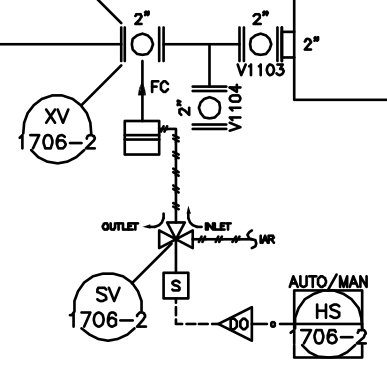
\includegraphics[width=0.38\linewidth]{../../figures/PInD-ex2.png}};

    %\foreach \x in {-2, -1,...,2} \draw[thin, black!30] (\x,-2) to (\x, 2);
    %\foreach \y in {-2, -1,...,2} \draw[thin, black!30] (-2,\y) to (2,\y);

    \node[coordinate,pin=190:{On/Off valve}] at (-1.7,0.8) {};
    \node[coordinate,pin={[pin distance=3cm]170:{Fail closed}}] at (-0.4,1.2) {};
    \node[coordinate,pin={[pin distance=3cm]0:{Pneumatic cylinder (piston)}}] at (-0.6,0.6) {};
    \node[coordinate,pin=190:{3/2 valve}] at (-0.5,-0.6) {};
    \node[coordinate,pin=10:{Compressed air}] at (0.3,-0.6) {};
    \node[coordinate,pin={[pin distance=1.4cm]-100:{Solenoid}}] at (-0.15,-1.1) {};
    \node[coordinate,pin={[pin distance=1cm]-80:{Digital output}}] at (0.55,-1.8) {};
    \node[coordinate,pin={[pin distance=1cm] 00:{Hand switch}}] at (1.8,-1.5) {};
    \node[coordinate,pin={[pin distance=1cm] 110:{Ball valve, 2in diam}}] at (-0.7,1.8) {};
    \node[coordinate,pin={[pin distance=1cm] 70:{Flanged connection}}] at (-0.4,1.8) {};
    \node[coordinate,pin={[pin distance=2cm] 220:{Solenoid valve}}] at (-1.2,-1.4) {};
  \end{tikzpicture}
\end{center}

\section*{Example 3}
\begin{center}
  \begin{tikzpicture}
    \tikzset{
      every pin/.style={pin distance=2cm,fill=blue!20!white,rectangle,rounded corners=3pt,font=\small,
      align=left},
    small dot/.style={fill=black,circle,scale=0.3},
  }

    \node {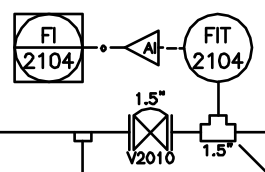
\includegraphics[width=0.28\linewidth]{../../figures/PInD-ex3.png}};

    %\foreach \x in {-2, -1,...,2} \draw[thin, black!30] (\x,-2) to (\x, 2);
    %\foreach \y in {-2, -1,...,2} \draw[thin, black!30] (-2,\y) to (2,\y);

    \node[coordinate,pin=170:{Flow indicator\\on computer screen\\in control room}] at (-1.2,0.8) {};
    \node[coordinate,pin={[pin distance=2cm]-90:{Diaphragm valve\\1.5in diam}}] at (0.2,-0.5) {};
    \node[coordinate,pin={[pin distance=1cm] 90:{Analog input}}] at (0.2,.6) {};
    \node[coordinate,pin={[pin distance=1cm] 00:{Flow indicate transmitter\\located in field}}] at (1.1,.8) {};
    \node[coordinate,pin={[pin distance=2cm] 220:{T-connection}}] at (-0.8,-0.8) {};
  \end{tikzpicture}
\end{center}

\newpage
\section*{Example 4}
\begin{center}
  \begin{tikzpicture}
    \tikzset{
      every pin/.style={pin distance=2cm,fill=blue!20!white,rectangle,rounded corners=3pt,font=\small,
      align=left},
    small dot/.style={fill=black,circle,scale=0.3},
  }

    \node {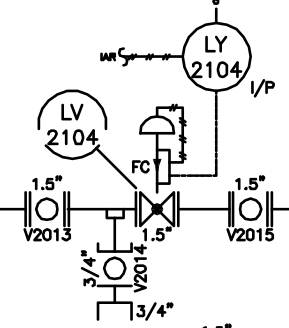
\includegraphics[width=0.28\linewidth]{../../figures/PInD-ex4.png}};

    %\foreach \x in {-2, -1,...,2} \draw[thin, black!30] (\x,-2) to (\x, 2);
    %\foreach \y in {-2, -1,...,2} \draw[thin, black!30] (-2,\y) to (2,\y);

    \node[coordinate,pin=170:{Level control valve}] at (-1.2,0.8) {};
    \node[coordinate,pin=170:{Flanged connection}] at (-1.4,-0.5) {};
    \node[coordinate,pin={[pin distance=2cm]-60:{Globe valve\\1.5in diam}}] at (0.2,-0.5) {};
    \node[coordinate,pin={[pin distance=2.6cm]-30:{Fail closed}}] at (0,0) {};
    \node[coordinate,pin={[pin distance=1cm] 100:{Compressed air (pneumatic signal)}}] at (0,1.25) {};
    \node[coordinate,pin={[pin distance=1cm] 10:{Level compute/relay\\I/P converter\\located in field}}] at (1.1,1.3) {};
    \node[coordinate,pin={[pin distance=1cm] 0:{Current to pneumatic conversion}}] at (1.6,0.9) {};
    \node[coordinate,pin={[pin distance=2cm] -10:{Pneumatically actuated valve}}] at (.1,0.5) {};
    \node[coordinate,pin={[pin distance=2cm] 220:{Ball valve\\1.5in diam}}] at (-1.1,-0.7) {};
  \end{tikzpicture}
\end{center}


\end{document}
